% Drawing 76/01-6 -- folder 76, batch 01, archive page 11 (PDF page 12).
% Transcription: en bas à droite, une figure : un arc qui monte puis file vers la droite jusqu'à une pointe, et sous lui quatre traits parallèles obliques ; sous les traits, les chiffres $0$, $1$, $2$, $3$ ; plus bas $D_1$, $D_2$, et au-dessus de l'arc « — $D_3$ ».
% Kind: arc with four parallel strokes numbered 0 to 3. Method 2 (schematic redraw from the facsimile). Status: ok.
% Notes: As on the page: the arc rising from the lower left and running to a tip at the far right; four parallel oblique strokes under it, each starting near the left part of the arc and stopping short of its upper part, the lower ones longer; the digits 0, 1, 2, 3 in a row under the strokes; D_1 and D_2 below them; « -- D_3 » above the arc. Left out: « 1, 1 + 1, 1 + 2 » with the vertical equality sign and the 2, at the right, and the formula below, which the transcription gives; the lattice arrows at the upper left of the crop (other drawings). The transcription's note speaks of an arrow towards D_3: the stroke before D_3 is a short dash. Redrawn 2026-11-12 (issue 128): to check again.
% Coordinates: 1 unit = 1 mm = 1/100 of the crop width (bbox in page fractions: [0.46, 0.7, 0.96, 0.86]).
% Redrawn by Claude (claude-fable-5-2), issue #128, 2026-11-12; not checked by a human; not compiled (no TeX in the session).
% Rights: reproduces part of the work -- behind RENDER_TRANSCRIPTS, never published by itself.
\documentclass[tikz,border=3pt]{standalone}
\usepackage{amsmath,amssymb}
\usetikzlibrary{patterns,arrows.meta}
\tikzset{pencil/.style={black!45}, struck/.style={black!35}, mpt/.style={circle,draw,inner sep=1.3pt}, pt/.style={circle,fill,inner sep=0.9pt}, opt/.style={circle,draw,fill=white,inner sep=1.1pt}}
\begin{document}
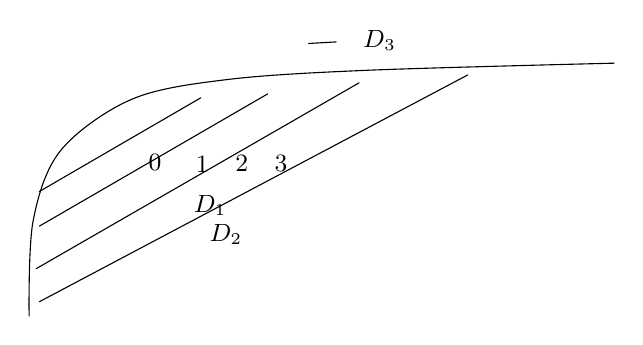
\begin{tikzpicture}[x=1mm,y=1mm,line cap=round,line join=round,font=\scriptsize]
\draw plot[smooth, tension=0.55] coordinates {(7,-45) (7.5,-33) (11,-24) (20,-17.5) (32,-15) (50,-13.8) (81.3,-12.9)};
\draw (8.3,-29.2) -- (28.8,-17.3);
\draw (8.3,-33.6) -- (37.3,-16.8);
\draw (7.9,-39) -- (48.9,-15.4);
\draw (8.3,-43.2) -- (62.7,-14.4);
\node[inner sep=1pt] at (23,-25.5) {\small $0$};
\node[inner sep=1pt] at (29,-25.8) {\small $1$};
\node[inner sep=1pt] at (34,-25.6) {\small $2$};
\node[inner sep=1pt] at (39,-25.6) {\small $3$};
\node[inner sep=1pt] at (30,-31) {\small $D_1$};
\node[inner sep=1pt] at (32,-34.7) {\small $D_2$};
\draw (42.5,-10.4) -- (46,-10.2);
\node[inner sep=1pt] at (51.5,-10) {\small $D_3$};
\end{tikzpicture}
\end{document}
